\chapter{Introduction}

Drug (Figure \ref{Introduction:Drugs}) discovery is an expensive and long-term business. It takes about US\$1.8 billion over 13.5 years to develop a new drug \citep{716}.

\begin{figure}[h]
\centering
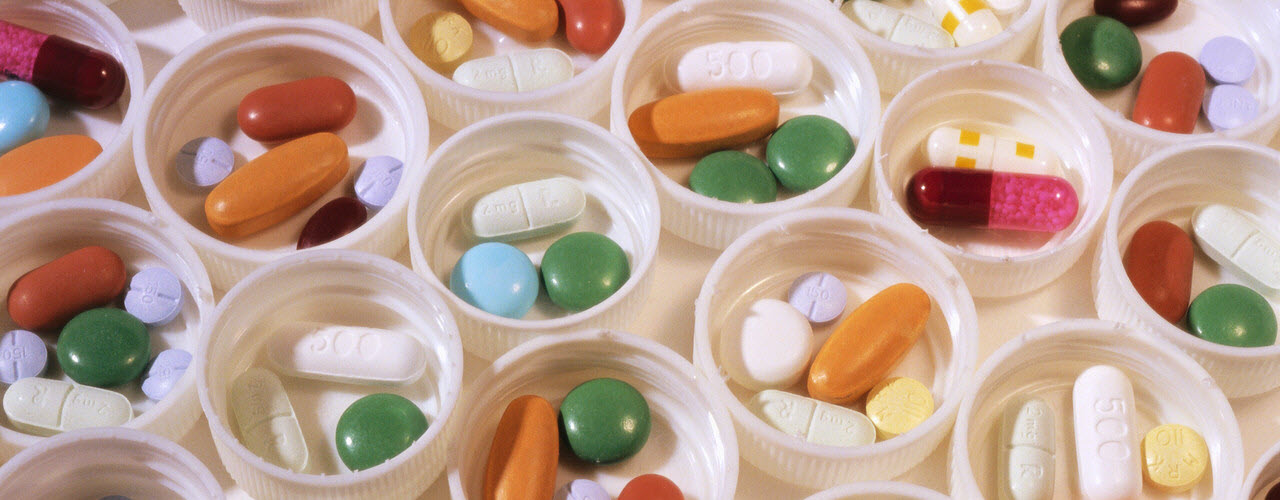
\includegraphics[width=\textwidth]{Introduction/Drugs.jpg}
\caption{Drugs.}
\label{Introduction:Drugs}
\end{figure}

\section{Motivation}

Drug discovery via biological and chemical means alone are both cost- and time-inefficient. It highlights the need for cheaper and faster method, and computer-aided drug discovery thus comes into the scene. Over recent decades, researchers have developed countless tools and utilities, and more are constantly emerging. We have surveyed those tools and utilities, and summarized the major problems they suffer from. Generally speaking, they
\begin{enumerate}
\item are commercially available, selling at a price that most small enterprises and academic researchers cannot afford,
\item are proprietary, making it difficult for others to learn inner implementation techniques and locate possible bugs,
\item conform to different standards and formats, resulting in loss of information during format conversion,
\item require intensive and tedious configurations and lack fruitful documentations, a great obstacle for program setup,
\item run very slowly, using old-fashioned, blocking, single-threaded, low-performance programming style,
\item are declared dead immediately upon their initial release due to zero maintenance afterward.
\end{enumerate}
Therefore, we are going to address these shortcomings.

\section{Objective}

We aim to develop a novel and concise computational framework for modern drug discovery. Our framework shall
\begin{enumerate}
\item be free to the general public so that everyone can obtain it,
\item be released under permissive open source licenses so that everyone can study it,
\item be designed in conformance to a uniform and well-accepted standard so that everyone can use it with ease,
\item provide a SaaS (Software as a Service) platform with a responsive web site so that everyone can play with it,
\item utilize multithreading and GPU acceleration to boost performance so that everyone can really benefit from it,
\item track bugs, absorb user feedback, and release new versions regularly so that everyone can keep using it.
\end{enumerate}

\section{Contributions}

Figure \ref{Introduction:Contributions} and table \ref{Introduction:Progress} summarize our contributions and roughly estimate the current progress of our projects and case studies.

\begin{figure}
\centering
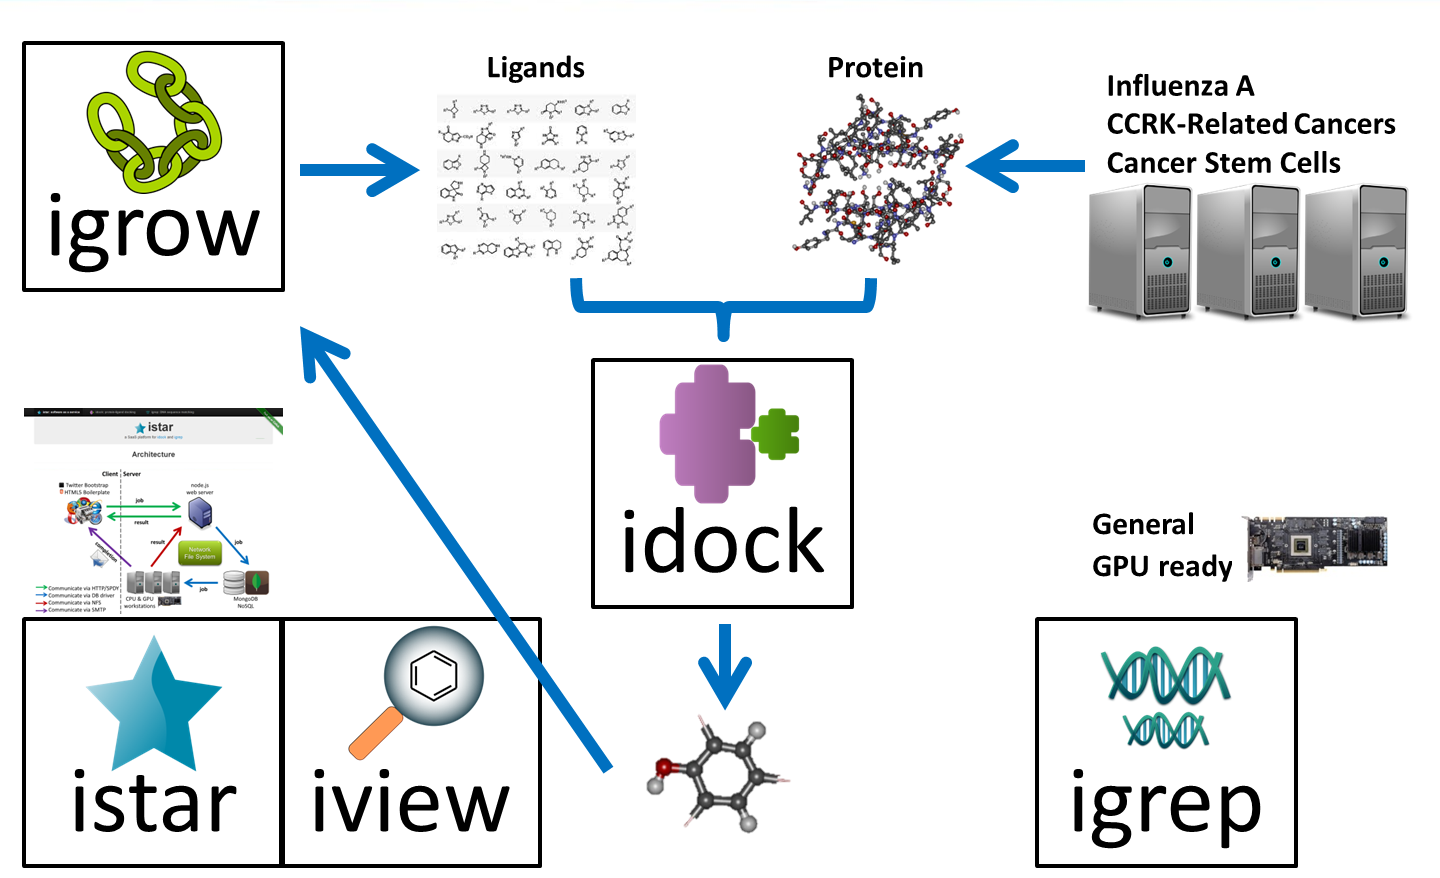
\includegraphics[width=\textwidth]{Introduction/Contributions.png}
\caption{An overall picture of our contributions.}
\label{Introduction:Contributions}
\end{figure}

\begin{table}
\centering
\begin{tabular*}
{\linewidth}
{@{\extracolsep{\fill}}p{0.85\textwidth}r}
\toprule
Projects / Case studies & Progress \\
\midrule
\textbf{idock 1.0: Protein-Ligand Docking} \citep{1153}. & 100\% \\
We have implemented built-in support for massive docking, a novel thread pool for parallel execution, automatic detection of inactive torsions, a revised numerical approximation model, and full reproducibility with precompiled executables for five operating systems, source code, use cases and API documentations. & \\
\textbf{idock 2.0: Protein-Ligand Docking}. & 100\% \\
We have implemented support for a total of 25 chemical elements, support for gzip/bzip2 compression, automatic docking recovery, detection of putative hydrogen bonds, per-atom binding affinity and ligand efficiency output, neat progress report, and many other great features. & \\
\textbf{istar: SaaS Platform} (submitted to a journal) & 100\% \\
We have developed istar as a SaaS (Software as a Service) platform for running programs online, and ported idock and igrep onto istar, featuring ligand filtering and previewing, progress monitoring in real time, innovative two-phase docking, slice-level parallelism, supplier list output, and GPU acceleration. & \\
\textbf{idock 3.0: GPU Acceleration} & 5\% \\
We have surveyed the latest GPU architectures codenamed GK104 and Tahiti, and observed thread behaviors and identified program hotspots of idock 2.0. We propose to support both CUDA and OpenCL in idock 3.0. & \\
\textbf{idock 4.0: Ligand Synthesis} & 30\% \\
We are developing igrow for computational synthesis of potent ligands, utilizing idock as the backend docking engine. We propose to integrate igrow into idock 4.0 to realize data caching and partial docking. We will exploit click chemistry for realistic synthetic feasibility, and implement dual-ligand docking. & \\
\textbf{Case Study of Influenza A Virus H1N1} & 90\% \\
We have identified the nucleoprotein and the RNA polymerase subunits PA and PB2 as druggable protein targets, and spent six months in running idock to test over 10 million ligands. We are now seeking for appropriate vendors. & \\
\textbf{Case Study of CCRK-Related Cancers} & 90\% \\
We have identified CCRK (Cell Cycle-Related Kinase) to involve in glioblastoma multiforme carcinogenesis, ovarian carcinomas and hepatocarcinogenesis. We have built a homologous model for CCRK and executed idock to test about 5 thousand approved drugs. We are now seeking for appropriate vendors. & \\
\textbf{Case Study of Cancer Stem Cells} & 0\% \\
We have identified the Wnt/$\beta$-catenin signaling pathway. Unfortunately, we could find neither a crystal structure of Wnt1 nor an appropriate template for homology modeling. We will explore other relevant signaling pathways. & \\
\bottomrule
\end{tabular*}
\caption{Contributions and progress of our projects and case studies.}
\label{Introduction:Progress}
\end{table}

\section{Outline}

Chapter 2 serves as a literature survey on computer-aided drug discovery. Chapter 3 presents idock for protein-ligand docking. Chapter 4 presents istar as a SaaS platform. Chapter 5 describes our proposal about idock 3.0, idock 4.0, iview and other ideas. Chapter 6 introduces our real-life drug discovery case studies. Chapter 7 concludes the thesis proposal. Appendix A lists my publications.

\chapterend
